%%%%%%%%%%%%%%%%%%%%%%%%%%%%%%%%%%%%%%%%%
% FRI Data Science_report LaTeX Template
% Version 1.0 (28/1/2020)
% 
% Jure Demšar (jure.demsar@fri.uni-lj.si)
%
% Based on MicromouseSymp article template by:
% Mathias Legrand (legrand.mathias@gmail.com) 
% With extensive modifications by:
% Antonio Valente (antonio.luis.valente@gmail.com)
%
% License:
% CC BY-NC-SA 3.0 (http://creativecommons.org/licenses/by-nc-sa/3.0/)
%
%%%%%%%%%%%%%%%%%%%%%%%%%%%%%%%%%%%%%%%%%


%----------------------------------------------------------------------------------------
%	PACKAGES AND OTHER DOCUMENT CONFIGURATIONS
%----------------------------------------------------------------------------------------
\documentclass[fleqn,moreauthors,10pt]{ds_report}
\usepackage[english]{babel}

\graphicspath{{fig/}}




%----------------------------------------------------------------------------------------
%	ARTICLE INFORMATION
%----------------------------------------------------------------------------------------

% Header
\JournalInfo{FRI Natural language processing course 2024}

% Interim or final report
\Archive{Project report} 
%\Archive{Final report} 

% Article title
\PaperTitle{LLM Prompt Strategies for Commonsense-Reasoning Tasks} 

% Authors (student competitors) and their info
\Authors{Žan Počkar, Amer Mujagić, and Ivan Nikolov}

% Advisors
\affiliation{\textit{Advisors: Aleš Žagar}}

% Keywords
\Keywords{Prompt Strategies, Prompt Evaluation}
\newcommand{\keywordname}{Keywords}


%----------------------------------------------------------------------------------------
%	ABSTRACT
%----------------------------------------------------------------------------------------

\Abstract{
Large Language Models (LLMs) have made significant advancements through extensive training, yet enhancing their commonsense reasoning remains challenging. This report evaluates four prompting strategies for their effectiveness in improving LLMs' commonsense reasoning using a subset of the aNLI, Physical IQa, and WinoGrande datasets. Our findings show that Few-Shot prompting significantly outperforms other methods, achieving over 20\% higher accuracy on the aNLI dataset. Conversely, Chain of Thought with Hints underperforms compared to zero-shot prompting. These results highlight the need for more sophisticated evaluation metrics and the potential of structured prompting techniques to enhance LLM performance on commonsense tasks. Future work will refine these techniques and expand evaluation to additional models and strategies.
}

%----------------------------------------------------------------------------------------

\begin{document}

% Makes all text pages the same height
\flushbottom 

% Print the title and abstract box
\maketitle 

% Removes page numbering from the first page
\thispagestyle{empty} 

%----------------------------------------------------------------------------------------
%	ARTICLE CONTENTS
%----------------------------------------------------------------------------------------

\section*{Introduction}
Large Language Models (LLMs) have demonstrated remarkable progress in various tasks when provided with extensive training material. However, enhancing their commonsense reasoning abilities remains a significant challenge. Commonsense reasoning, which entails making judgments based on everyday knowledge and experiences, is an essential aspect of human intelligence, and incorporating this capability into LLMs is a complex endeavor.

In this paper, we compare four prompting strategies using the same problem set and model to evaluate their performance. Our flexible evaluation framework is designed to accommodate multiple models and strategies in the future and serves as a simple blueprint for adding similar strategies. We employed a subset of aNLI, Physical IQa, and WinoGrande datasets, inspired by the Rainbow dataset, using the first 300 questions as a proof of concept and a good general idea of their comparative performance. The primary objective of this paper is to demonstrate the effectiveness of our evaluation framework and provide a roadmap for comparing different prompt strategies on various LLMs.

%------------------------------------------------
\section*{Problem}

\subsection*{Commonsense reasoning}
Commonsense reasoning in Large Language Models (LLMs) is a complex problem due to the implicit and context-dependent nature of commonsense knowledge. For instance, consider the sentence, “The ice cream was too hot to eat.” Humans intuitively understand this sentence is likely incorrect because ice cream is typically cold. However, an LLM might not flag this as an anomaly unless it has been explicitly trained on similar examples or has learned to associate certain objects with their typical properties.

\subsection*{Prompt generation}
The idea of generating prompts from prompts seems straightforward, and for the most part, depending on the technique, it can be. However, comparing techniques based on these prompts remains a challenge. It is difficult to quantify the impact of prompt modifications on complexity or simplicity when adapting them to fit specific techniques. This issue may result in a biased comparison between techniques. We tried to mitigate this problem by selecting diverse datasets, but it was challenging to quantify the impact in a meaningful way. As a result, our findings should be interpreted while considering that changing the prompts might have simplified them, potentially biasing the comparison between techniques. This is particularly relevant for Chain of Thought with hints, where automatically generated hints were often extremely directly connected to the answer.


\section*{Prompting Techniques}
Prompts techniques are the proposed input structures that guide LLMs to produce outputs with the desired form and content quality. That is, to simplify, we can say that we use different prompting techniques to "program" LLM inputs by following specific patterns in order to obtain an output. \cite{prompttechniques}

\subsection*{Few-shot and zero-shot Prompting}
Few-shot prompting \cite{Few-shot} is a technique that involves providing a prompt along with a limited number of demonstrations to help guide the Large Language Model (LLM) in understanding and performing a specific task. In contrast to zero-shot prompting, where no demonstrations are used, few-shot prompting allows for a more nuanced understanding by providing examples that showcase the desired output.

As illustrated in Figure \ref{fig:few-shot}, few-shot prompting lies between zero-shot and one-shot prompting in terms of the number of demonstrations provided. By including examples, the LLM can better grasp the context and the expected results. However, the challenge lies in balancing the complexity of the prompt and the number of demonstrations provided. Too few examples might not provide sufficient guidance, while too many may overfit the LLM to the specific examples and hinder generalization.
Overall, few-shot prompting offers a flexible approach to enhancing LLM performance by combining the simplicity of natural language instructions with the additional context provided by demonstrations.

\begin{figure}[!h]
    \centering
    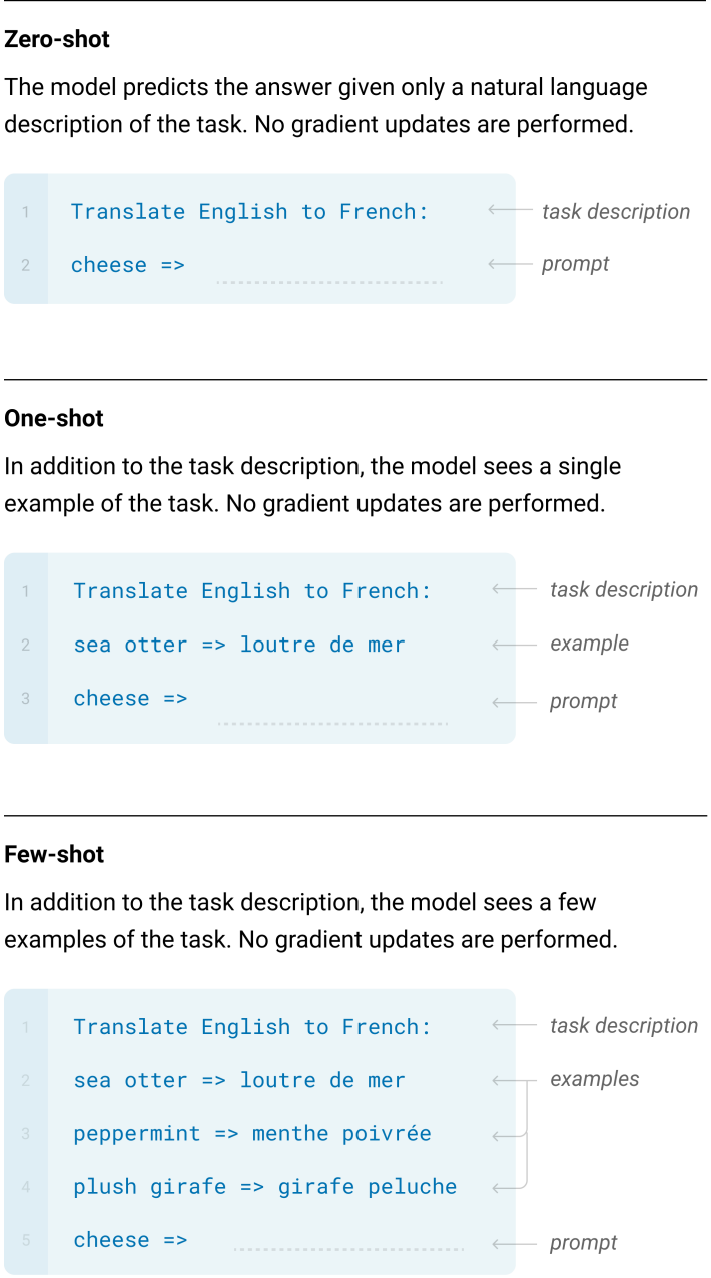
\includegraphics[width=0.6\linewidth]{fig/few-shot-new.png}
    \caption{Zero-shot, one-shot, and few-shot prompts}
    \label{fig:few-shot}
\end{figure}


\subsection*{Chain of Thought}
Chain of Thought (CoT) \cite{CoT} prompting involves adding a series of intermediate reasoning steps to the intended task. It has been shown to improve performance in more complex prompts.
These intermediate reasoning steps can be thought of as giving an answer to a similar problem but with detailed steps on how to get to that answer as shown in Figure 1. This is similar to few-shot prompting, which also provides examples of answers to similar questions, however few-shot prompts include less detail that is they usually provide only questions and answers, no intermediate reasoning steps in between. \cite{CoT}
An example of Chain of Thought prompting can be seen in Figure \ref{fig:cot}
\begin{figure}[!h]\centering
	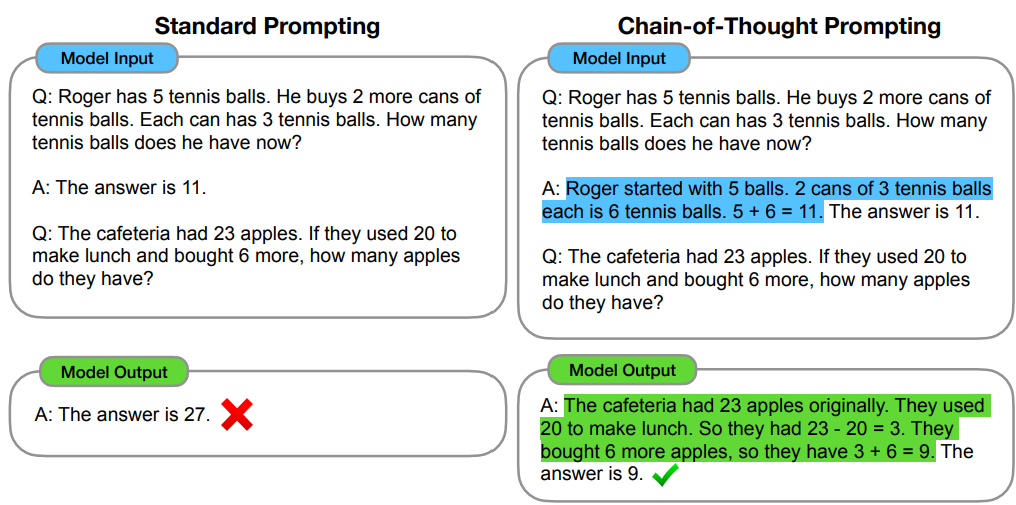
\includegraphics[width=0.8\linewidth]{Example_CoT.png}
	\caption{Example of a Chain of Thought prompt versus a regular prompt}
	\label{fig:cot}
\end{figure}

\subsubsection*{Chain of Thought with hints}
Chain of Thought with hints other than the standard thought process contains also a hint pointing to the correct answer. The hint should not be too obvious to answer the question directly (because then the prompt uses any usefulness) but not too vague so it confuses the model.



\section*{Datasets}
Because commonsense reasoning is a complex topic and encompasses a wide collection of different tasks, it is difficult to generate a dataset that will evaluate the model's generalization abilities.

The Winograd schema challenge \cite{levesque2012winograd} was the standard for testing the commonsense reasoning, however from 2019 it is considered defeated since numerous transformer-based models achieved over 90\% accuracy. \cite{beaten_winograd}
For that reason, we will use more recent and challenging datasets.

On the one side, we have different SOTA methods \cite{CoT} evaluated on task specific datasets like GSM8K \cite{GSMK8}. This dataset focuses on linguistically diverse grade school math problems created by human problem writers.

On the other side, there are benchmarks that combine multiple commonsense datasets. For this project we will use Rainbow which is a suite of commonsense benchmarks that contain multiple choice question-answering datasets.
For our experiments, we selected the following three datasets from Rainbow

\begin{itemize}
    \item $\alpha$NLI \cite{alphaNLI} - tests abductive reasoning in narratives. Models need to find the best explanation among the presented options connecting a beginning and ending;
    \item Physical IQa \cite{Bisk2020} — question answering benchmark for physical commonsense.
    \item WinoGrande \cite{WinoGRANDE} — large-scale collection of Winograd schema-inspired problems that test reasoning about social and physical interactions.
\end{itemize}

% Other possibilities for testing commonsense reasoning are the GLUE \cite{GLUE} and SuperGLUE \cite{supeglue} datasets, which are benchmarks for general language understanding systems.

\section*{Methodology}
Our evaluation pipeline consists of three main components. First, we modify the datasets to obtain hints and examples for few-shot prompts. Second, we generate results using these modified prompts. Finally, we evaluate the results and compare them.

\subsection*{Prompt Modification}
We utilized the DSPy framework's ChainOfThought and Predict modules to modify the prompts to fit a given strategy. Since the framework already contained the ChainOfThought and ChainOfThoughtWithHints modules, we decided to use them directly for prompt generation. However, our datasets lacked hints and examples for our Few-shot prompts. To generate the examples and hints, we employed the Mistral-7B model and the Predict module. We used custom signatures fine-tuned to each dataset's structure to maximize the effectiveness of the models. These signatures only explained the structure of the prompt and the expected output, without any additional information about the prompt. We made 1 signature per output type (that is examples or hint) and per module, so a total of 6 custom signatures for this part of the assignment.

\subsection*{Answer Generation}
We once again utilized the DSPy ChainOfThought, Predict, and ChainOfThoughtWithHints modules to generate answers for the prompts using different techniques. For Few-shot prompts, we used the Predict module, incorporating the examples into the questions themselves. We created custom signatures for each dataset, as their structures varied slightly. We used one signature per module for three of the strategies and a separate signature for Few-shot prompts due to their additional examples in the questions.

\subsection*{Data preprocessing}
Before we could compare the generated answers, we firstly need to process the data into a singular form. We agreed to use JSON format for our data, but even with the set format some prompting techniques field the format incorrectly. To prepare the data we mostly had to transform string into integers, add indexing and in the few cases we actually need to find the given answers in the raw field of the format.

\section*{Results}
\subsection*{Evaluation}
We are currently performing evaluation of the models answers with two different methods. In the first method where the model has to select between choices and then give his answer we use a simple comparison algorithm. If the model gives multiple answers, we count up the choices and use his most often given answer as the answer we use for comparison. The comparison algorithm is then a simple checker which has the list of correct answers. The checker compares the question id and content from the correct list with those give by the model. And then prints the results. This give are hard data we can compare.

In the second approach we wore more interested in the model's reasoning and especially on the question answered wrongly, so instead of just comparing selected numbers we used a different large language module google/Gemma to compare the given answers and decide on the most correct one. In this method, we are using an uncased BERT model to generate the embedding and calculate the cosine similarity between the correct answer and the given one. As an additional layer of grading we are comparing cosine similarity with Word2Vec model to better determine the meaning of the sentence these two scores are then combine and if the answer pass the threshold of correctness we are considering the answer as correct. This model also supports comparison of different techniques, and not just direct comparison between the result and the technique. This way we can determine which technique is closer to the right answer even if this particular answer is incorrect. Sadly, even with all the steps we took to produce reproducible results, we just couldn't get the model to give consistent results. So in the end in the name of reproducibility of results we only used the first method in our report.


\subsection*{Results}
The results were not all as expected, while we did generally see an improvement when using prompting techniques the improvement varied very much from small to big and in a few cases even worsening performance.

The best result we got from the Winograd and the Anli datasets, where we can see improvements with using the chain of thought and the few shot prompting techniques. But we see the worst performance with the chain of thought with hints techniques performance.



While the results for Physical dataset do follow the general trend, the overall performance of the model was very bad. We still don't understand, even if we used a lot of our time to troubleshoot it


The last image clearly shows that the techniques have effect non withstanding which dataset we used, but that they are more effective for certain datasets.

\begin{figure}[!h]
    \centering
    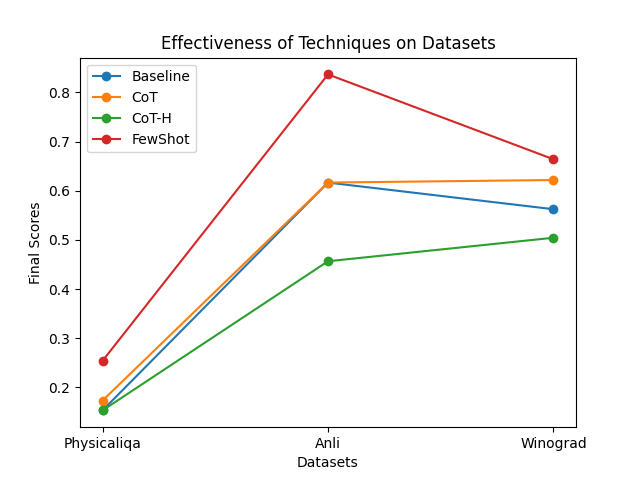
\includegraphics[width=0.75\linewidth]{Effectiveness_of_Techniques_on_Datasets.png}
    \caption{Technique Effectivnes across Datasets}
    \label{line-graph}
\end{figure}
 

\section*{Discussion}
The framework serves as a valuable blueprint, even though the results might not fully represent the techniques themselves but rather showcase the DSPy framework's implementation. Despite following the official documentation, some results were weaker than anticipated. Notably, Chain of Thought, especially with hints, was expected to outperform Few-Shot examples, but it did not always yield the desired outcome, even when the generated hints were evident.

The framework's modules, while being easy to use, provided answers in a format that was difficult to parse, often mixing random questions and answers in the same section. This structure made it challenging to differentiate and extract relevant information automatically.

Additional challenges included the time needed to generate results and limited resources. These factors might have impacted the quality of the results. Running the experiments multiple times would help account for the inherent uncertainty of LLMs and further refine the analysis.

In conclusion, the framework demonstrates significant potential as a blueprint. Future work should focus on investigating and optimizing the effectiveness of these prompt strategies while addressing the identified issues.  Additionally, further investigation into utilizing built-in prompt optimization mechanisms could enhance the framework's overall utility.
 This approach will enable a more comprehensive assessment of the framework's performance and its ability to contribute to the ongoing advancement of LLM prompting techniques.

 
%----------------------------------------------------------------------------------------
%	REFERENCE LIST
%----------------------------------------------------------------------------------------
\bibliographystyle{unsrt}
\bibliography{report}


\end{document}